\documentclass[12pt]{article}
\usepackage[margin=1in]{geometry}
%\UseRawInputEncoding
\usepackage{amsmath,hyperref}
\usepackage[listings]{tcolorbox}

\definecolor{codegreen}{rgb}{0,0.4,0}
\definecolor{codegray}{rgb}{0.5,0.5,0.5}
\definecolor{codepurple}{rgb}{0.58,0,0.82}
\definecolor{backcolour}{rgb}{0.95,0.95,0.92}

\lstdefinestyle{mystyle}{
    language=R,
    backgroundcolor=\color{backcolour},   
    commentstyle=\color{codegreen},
    keywordstyle=\color{magenta},
    numberstyle=\tiny\color{codegray},
    stringstyle=\color{codepurple},
    basicstyle=\ttfamily\normalsize,
    breakatwhitespace=false,         
    breaklines=true,                 
    captionpos=b,                    
    keepspaces=true,                 
    numbers=left,                    
    numbersep=5pt,                  
    showspaces=false,                
    showstringspaces=false,
    showtabs=false,                  
    tabsize=2,
    escapechar=|,
    frame=single
}

\lstset{style=mystyle}


\newcommand{\arrow}{\ensuremath{\rightarrow}}
\newcommand{\lst}[1]{\lstinline{#1}}

\title{csci297b Exercise 3\\Dataframes }
\date{}
\sloppy

\begin{document}
\maketitle

\begin{enumerate}

\centerline{\bf Part 1}


\item Log on to the RStudio Workbench Server. 
In the same project as the previous exercise, open a new R script called 
\verb|exercise_3|.
Make sure you include any metadata you feel is appropriate (title, description of task, date of script creation etc). Don’t forget to comment out your metadata with a \lstinline{#} at the beginning of the line.

\item Download all the data at once, found here: \url{https://alexd106.github.io/intro2R/data.html}

This will download a zip file to your local computer.  Do not decompress it.  

\item In Rstudio Workbench, under the Files tab, click the Upload button.  Browse to 
where you downloaded the zip file (usually "Downloads"), and select the 
\verb|all_data.zip| file.  This will upload and simultaneously unzip
the file into the filesystem on the server.

\item Still in the Files tab, there should now be a \verb|data| folder.  Open this folder
and click on the \verb|whaledata.xls|, and then "Import dataset".  Click again
on the "Import" button.

\item In the console you should now see the text:
\begin{lstlisting}
> library(readxl)
> whaledata <- read_excel("data/whaledata.xls")
> View(whaledata)                                                                        
\end{lstlisting}
RStudio has entered the R commands needed to load the dataset into a {\bf dataframe},
or a specialized kind of dataframe called a {\bf tibble}.  (More about this later)

\item
Instead of clicking the button, you could have entered these commands
in the console, or sourced them from a script.  Let's do that now.  In your
script for this exercise, enter the following:
\begin{lstlisting}
library(readxl)
whaledata <- read_excel("data/whaledata.xls")
View(whaledata)                                                                        
\end{lstlisting}
Now source the script into the console.  

Entering these commands into a script seems like more work.  But the
next time you want to deal with this script and this dataset, the commands
will load it for you.  You will {\em not} have to open the file browser,
locate the file, and click on it.  In the long run, opening the files you
need from the script is much more efficient than the "hunt-and-click"
that seems convenient the first time.

Get in the habit of making your scripts self-contained.  Loading
the script and pressing the "Source" button should do everything
necessary.

\item
The \verb|whaledata.xls| is an Excel spreadsheet.  A lot of data is stored in 
this format.  However, a lot of data is stored in text files, without the overhead
required by Excel.  

To see this, go back to your local computer's file browser, and navigate to
the \verb|all_data.zip| file, and unzip it (double-click and follow instructions).

Now navigate into the \verb|data| folder (on your local computer, where you
unzipped the file), and open the \verb|whaledata.xls| file with spreadsheet
software.  If you don't have Microsoft products, you can get excellent free
versions here: \url{https://www.libreoffice.org/discover/libreoffice/}

\item
In the spreadsheet software, select "Save As", and then save the file as a
{\bf Text CSV} file, called \verb|whaledata.csv|

First, examine the two files in your file browser, selecting "View\arrow Details",
and notice that the CSV file is less than a fifth the size of the XLS file,
4 KB instead of 28 KB.  Most data prepared for data analysis is in this format,
not in spreadsheet format, simply because spreadsheets waste a lot of space
on formatting and other matters not related to the data itself.

Now open the CSV file with a {\em text editor}, such as Notepad on Windows
or TextEdit on Macs or gedit on Unix.  Notice that the file is humanly readable,
with simple layout. 


\item
For contrast, open the XLS file with a text editor.  You get something like we see
in Figure \ref{xlsfile}.  

\begin{figure}
\begin{center}
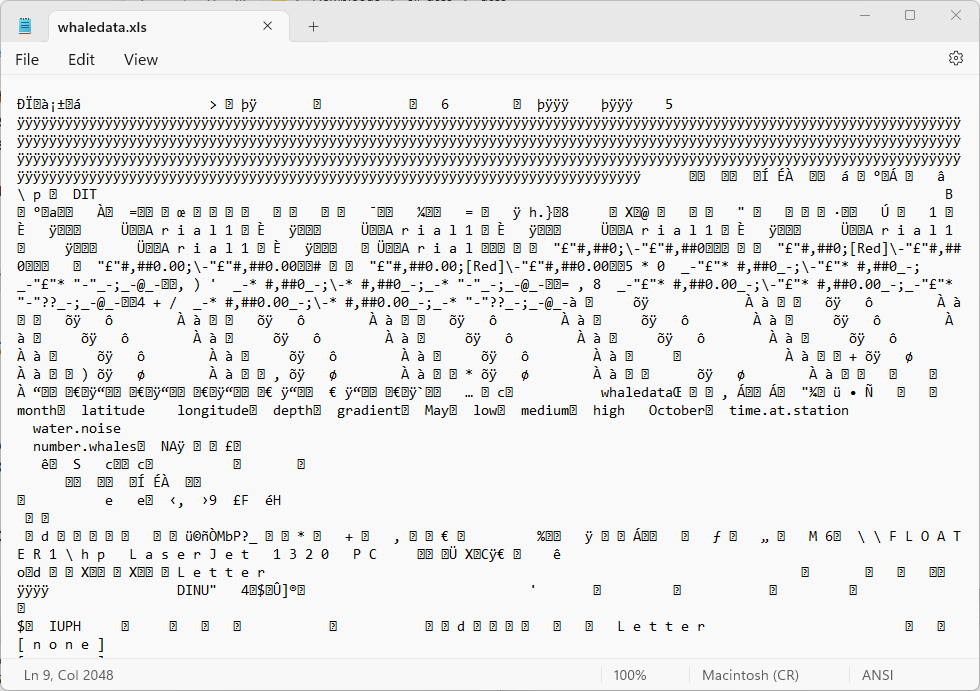
\includegraphics[width=0.66\textwidth]{xlsfile}
\end{center}
\caption{An XLS file opened with a text editor.}
\label{xlsfile}
\end{figure}

There are many disadvantages to the XLS format.  It is bulky, not humanly readable,
only readable by spreadsheet software.  Storing files in text format 
is preferable in nearly all cases.

\item
Upload the \verb|whaledata.csv| file to the same folder on the server.
Do {\em not} read the data by clicking on it.  Instead, enter the following
into your script and source it to the console:
\begin{lstlisting}
whale <- read.csv("data/whaledata.csv")
\end{lstlisting}

\verb|read.csv|is a variation on the \verb|read.table|
function.  Spend some time with \S 3.2.2 of the manual and also the 
help desk to learn more about this
important class of functions.

\item
After you load a data file, it's a good idea to look at it and make sure it has
loaded properly, and get a feel for what's there.  The RStudio command
added \lst{View(whaledata)} to its commands, which opens a spreadsheet-like
viewer in the editor panel.  You can try the same with your CSV data,
with \lst{View(whale)}.  Can you spot  some subtle differences between
the \lst{whaledata} dataset (loaded with \lst{read_excel}),
 and the \lst{whale} dataset (loaded with \lst{read.csv})?
 
 In what follows we will use the \lst{whale} dataset.

\item
Time for a quick description of the \verb|whaledata.txt| dataset to get your bearings. These data were collected during two research cruises in the North Atlantic in May and October 2003. During these two months the research vessel visited multiple stations (areas) and marine mammal observers recorded the number of whales (who doesn’t love whales!) at each of these stations. The time the vessel spent at each station was also recorded along with other site specific variables such as the latitude and longitude, water depth and gradient of the seabed. The researchers also recorded the ambient level of sub-surface noise with a hydrophone and categorised this variable into ‘low’, ‘medium’ or ‘high’. The structure of these data is known as a rectangular dataset (aka ‘tidy’ data by the cool kids) with no missing cells. Each row is an individual observation and each column a separate variable. The variable names are contained in the first row of the dataset (aka a header).

\item
The best way to learn a bit more about a dataframe enter the command
\begin{lstlisting}
str(whale)
\end{lstlisting}
 into your script and source it to the console.  You will 
see a display like this:
\begin{lstlisting}[basicstyle=\tiny]
> str(whale)
'data.frame':	100 obs. of  8 variables:
 $ month          : chr  "May" "May" "May" "May" ...
 $ time.at.station: int  1344 1633 743 1050 1764 580 459 561 709 690 ...
 $ water.noise    : chr  "low" "medium" "medium" "medium" ...
 $ number.whales  : int  7 13 12 10 12 10 5 8 11 12 ...
 $ latitude       : num  60.4 60.4 60.5 60.3 60.4 ...
 $ longitude      : num  -4.18 -4.19 -4.62 -4.35 -5.2 -5.22 -5.08 -5 -4.64 -4.84 ...
 $ depth          : int  520 559 1006 540 1000 1000 993 988 954 984 ...
 $ gradient       : int  415 405 88 409 97 173 162 162 245 161 ...
> 
 \end{lstlisting}
 This gives you important information about your data, including the names
 of the columns and the types of each, either numeric (num) or character (chr).

\item Also try \verb|summary(whale)| and explore what you get.

\centerline{\bf Part 2}

\item Summarising and manipulating dataframes is a key skill to acquire when learning R. Although there are many ways to do this, we will concentrate on using the square bracket [ ] notation which you used previously with vectors. The key thing to remember when using [ ] with dataframes is that dataframes have two dimensions (think rows and columns) so you always need to specify which rows and which columns you want inside the [ ] (see \S 3.4.1 for some additional background information and a few examples). Let's practice.

Put commands to find the answers to 
each of the following into your R script and source them to the console:
\begin{itemize}

\item
Extract all the elements of the first 10 rows and the first 4 columns of the whale dataframe and assign to a new variable called \lst{whale.sub}.
\item
Next, extract all observations (remember - rows) from the whale dataframe and the columns month, water.noise and number.whales and assign to a variable called \lst{whale.num}.
\item
Now, extract the first 50 rows and all columns form the original dataframe and assign to a variable \lst{whale.may} (there’s a better way to do this with conditional statements - see below).
\item
Finally, extract all rows except the first 10 rows and all columns except the last column. Remember, for some of these questions you can specify the columns you want either by position or by name. Practice both ways. Do you have a preference? If so why?

 \end{itemize}

\item In addition to extracting rows and columns from your dataframe by position you can also use conditional statements to select particular rows based on some logical criteria. This is very useful but takes a bit of practice to get used to (see Section 3.4.2 for an introduction). Extract rows from your dataframe (all columns by default) based on the following criteria (note: you will need to assign the results of these statements to appropriately named variables, I’ll leave it up to you to use informative names!):
\begin{itemize}
\item
at depths greater than 1200 m
\item
gradient steeper than 200 degrees
\item
water noise level of ‘low’
\item
water.noise level of ‘high’ in the month of ‘May’
\item
month of ‘October’, water noise level of ‘low’ and gradient greater than the median value of gradient (132)
\item
all observations from between latitudes 60.0 and 61.0 and longitudes -6.0 and -4.0
\item
all rows that do not have a water noise level of medium
\end{itemize}

\item A really neat feature of extracting rows based on conditional statements is that you can include R functions within the statement itself. To practice this, modify your answer to the gradient question to use the \lst{median()} function rather than hard coding the value 132.

\item However, when using functions in conditional statements you need to be careful. For example, write some code to extract all rows from the dataframe whale with depths greater than 1500 m and with a greater number of whales spotted than average (hint: use the \lst{mean()} function in your conditional statement). Can you see a problem with the output?   Check the help file for \lst{mean}
and in particular pay attention to the \lst{na.rm} parameter.


\item Although you have concentrated on using the square bracket [ ] notation to extract rows and columns from your dataframe, there are of course many other approaches. One such approach is to use the \lst{subset()} function. Look this function up in the manual or the help files.

Use the \lst{subset()} function to extract all rows in ‘May’ with a time at station less than 1000 minutes and a depth greater than 1000 m. Also use \lst{subset()} to extract data collected in ‘October’ from latitudes greater than 61 degrees but only include the columns month, latitude, longitude and number.whales.

\item Another useful way to manipulated your dataframes is to sort the rows based on the value of a variable (or combinations of variables). Rather counter-intuitively you should use the \lst{order()}
 function to sort your dataframes, not the \lst{sort()} function (see Section 3.4.3 of the Introduction to R book for an explanation). 
 

 
\item Now for something a little more complicated. Sort all rows in the whale dataframe by ascending order of depth within each level of water noise. The trick here is to remember that you can order by more than one variable when using the \lst{order()} function (see Section 3.4.3 again). Don’t forget to assign your sorted dataframe to a new variable with a sensible name. Repeat the previous ordering but this time order by descending order of depth within each level of water noise.

 \centerline{\bf Part 3}

\item Often, we would like to summarise variables by, for example, calculating a mean, median or counting the number of observations. To do this for a single variable it’s fairly straight forward :

 
\begin{lstlisting}
mean(whale$time.at.station)     # mean time at station
median(whale$depth)             # median depth
length(whale$number.whales)     # number of observations
\end{lstlisting}

 Perhaps more interestingly, you might want summarise one variable conditional on the level of another factor variable. For example, write some R code to calculate the mean number of whales sighted at each of the three levels of water noise (see Section 3.5 for a few hints). Next, calculate the median number of whales sighted at each level of water noise and for each month.

 

\item Another useful function for summarising dataframes is \lst{aggregate()}. Refer back to the book (search for aggregate) to look up how to use this function (or see ?aggregate). Use the \lst{aggregate()} function to calculate the mean of time at station, number of whales, depth and gradient for each level of water noise (don’t forget about that sneaky NA value). Next calculate the mean of time at station, number of whales, depth and gradient for each level of water noise for each month.
 

\item Knowing how many observations are present for each factor level (or combinations of factor levels) is useful to determine whether you have an adequate sample size (for subsequent modelling for example). Use the \lst{table()} function to determine the number of observations for each level of water noise (see Section 3.5 again for more information). Next use the same function to display the number of observations for each combination of water noise and month. (Optional): The \lst{xtabs()} function is very flexible for creating tables of counts for factor combinations (aka contingency tables). Take a look at the Introduction to R book, the help file or Google to figure out how to use the \lst{xtabs()} function to replicate your use of the table() function.


\item Ok, we have spent quite a bit of time (and energy) learning how to import and manipulate dataframes. The last thing we need to cover is how to export dataframes from R to an external file (see Section 3.6 of the book for more details). Let’s say you want to export the dataframe whale.num you created previously  to a file called \verb|whale_num.csv|. To do this you will need to use the 
\lst{write.table()} function. You want to include the the variable names in the first row of the file, but you don’t want to include the row names. Also, make sure the file is a comma delimited file. Once you have created your file,
download it to your local computer and try to open it in spreadsheet software.

\item Don’t to forget to save your R script. Since we put this script in the same project
as the last one, it should already be shared with your
instructor.

Close your Project by selecting File\arrow Close Project on the main menu.

\end{enumerate}
\end{document}